% Created by tikzDevice version 0.10.1 on 2017-11-22 12:37:21
% !TEX encoding = UTF-8 Unicode
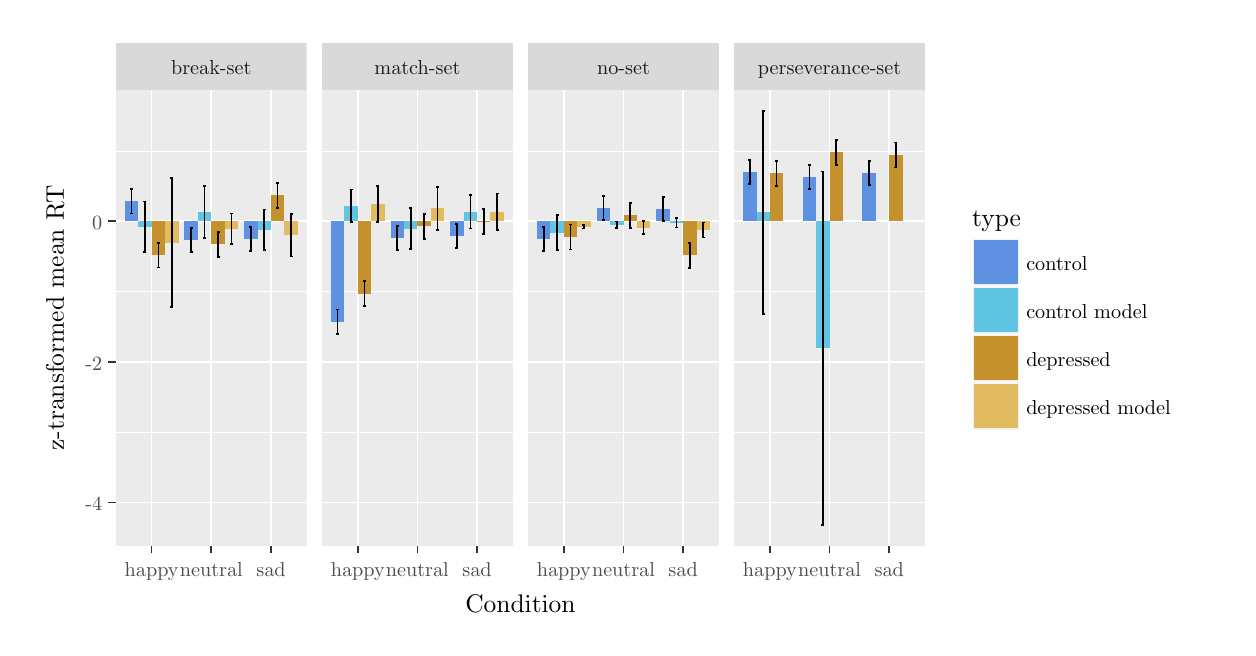
\begin{tikzpicture}[x=1pt,y=1pt]
\definecolor{fillColor}{RGB}{255,255,255}
\path[use as bounding box,fill=fillColor,fill opacity=0.00] (0,0) rectangle (433.62,216.81);
\begin{scope}
\path[clip] (  0.00,  0.00) rectangle (433.62,216.81);
\definecolor{drawColor}{RGB}{255,255,255}
\definecolor{fillColor}{RGB}{255,255,255}

\path[draw=drawColor,line width= 0.6pt,line join=round,line cap=round,fill=fillColor] (  0.00,  0.00) rectangle (433.62,216.81);
\end{scope}
\begin{scope}
\path[clip] ( 31.87, 29.59) rectangle (100.84,194.25);
\definecolor{fillColor}{gray}{0.92}

\path[fill=fillColor] ( 31.87, 29.59) rectangle (100.84,194.25);
\definecolor{drawColor}{RGB}{255,255,255}

\path[draw=drawColor,line width= 0.3pt,line join=round] ( 31.87, 70.68) --
	(100.84, 70.68);

\path[draw=drawColor,line width= 0.3pt,line join=round] ( 31.87,121.46) --
	(100.84,121.46);

\path[draw=drawColor,line width= 0.3pt,line join=round] ( 31.87,172.23) --
	(100.84,172.23);

\path[draw=drawColor,line width= 0.6pt,line join=round] ( 31.87, 45.29) --
	(100.84, 45.29);

\path[draw=drawColor,line width= 0.6pt,line join=round] ( 31.87, 96.07) --
	(100.84, 96.07);

\path[draw=drawColor,line width= 0.6pt,line join=round] ( 31.87,146.84) --
	(100.84,146.84);

\path[draw=drawColor,line width= 0.6pt,line join=round] ( 44.80, 29.59) --
	( 44.80,194.25);

\path[draw=drawColor,line width= 0.6pt,line join=round] ( 66.36, 29.59) --
	( 66.36,194.25);

\path[draw=drawColor,line width= 0.6pt,line join=round] ( 87.91, 29.59) --
	( 87.91,194.25);
\definecolor{fillColor}{RGB}{226,186,95}

\path[fill=fillColor] ( 49.65,139.17) rectangle ( 54.50,146.84);
\definecolor{fillColor}{RGB}{196,145,45}

\path[fill=fillColor] ( 44.80,134.60) rectangle ( 49.65,146.84);
\definecolor{fillColor}{RGB}{95,197,226}

\path[fill=fillColor] ( 39.95,144.85) rectangle ( 44.80,146.84);
\definecolor{fillColor}{RGB}{95,145,226}

\path[fill=fillColor] ( 35.10,146.84) rectangle ( 39.95,154.13);
\definecolor{fillColor}{RGB}{226,186,95}

\path[fill=fillColor] ( 71.21,144.11) rectangle ( 76.06,146.84);
\definecolor{fillColor}{RGB}{196,145,45}

\path[fill=fillColor] ( 66.36,138.46) rectangle ( 71.21,146.84);
\definecolor{fillColor}{RGB}{95,197,226}

\path[fill=fillColor] ( 61.51,146.84) rectangle ( 66.36,150.10);
\definecolor{fillColor}{RGB}{95,145,226}

\path[fill=fillColor] ( 56.66,140.16) rectangle ( 61.51,146.84);
\definecolor{fillColor}{RGB}{226,186,95}

\path[fill=fillColor] ( 92.76,141.83) rectangle ( 97.61,146.84);
\definecolor{fillColor}{RGB}{196,145,45}

\path[fill=fillColor] ( 87.91,146.84) rectangle ( 92.76,156.26);
\definecolor{fillColor}{RGB}{95,197,226}

\path[fill=fillColor] ( 83.06,143.81) rectangle ( 87.91,146.84);
\definecolor{fillColor}{RGB}{95,145,226}

\path[fill=fillColor] ( 78.21,140.45) rectangle ( 83.06,146.84);
\definecolor{drawColor}{RGB}{0,0,0}

\path[draw=drawColor,line width= 0.6pt,line join=round] ( 51.54,162.38) --
	( 52.62,162.38);

\path[draw=drawColor,line width= 0.6pt,line join=round] ( 52.08,162.38) --
	( 52.08,115.96);

\path[draw=drawColor,line width= 0.6pt,line join=round] ( 51.54,115.96) --
	( 52.62,115.96);

\path[draw=drawColor,line width= 0.6pt,line join=round] ( 46.69,139.11) --
	( 47.77,139.11);

\path[draw=drawColor,line width= 0.6pt,line join=round] ( 47.23,139.11) --
	( 47.23,130.10);

\path[draw=drawColor,line width= 0.6pt,line join=round] ( 46.69,130.10) --
	( 47.77,130.10);

\path[draw=drawColor,line width= 0.6pt,line join=round] ( 41.84,153.97) --
	( 42.92,153.97);

\path[draw=drawColor,line width= 0.6pt,line join=round] ( 42.38,153.97) --
	( 42.38,135.73);

\path[draw=drawColor,line width= 0.6pt,line join=round] ( 41.84,135.73) --
	( 42.92,135.73);

\path[draw=drawColor,line width= 0.6pt,line join=round] ( 36.99,158.58) --
	( 38.07,158.58);

\path[draw=drawColor,line width= 0.6pt,line join=round] ( 37.53,158.58) --
	( 37.53,149.68);

\path[draw=drawColor,line width= 0.6pt,line join=round] ( 36.99,149.68) --
	( 38.07,149.68);

\path[draw=drawColor,line width= 0.6pt,line join=round] ( 73.09,149.69) --
	( 74.17,149.69);

\path[draw=drawColor,line width= 0.6pt,line join=round] ( 73.63,149.69) --
	( 73.63,138.52);

\path[draw=drawColor,line width= 0.6pt,line join=round] ( 73.09,138.52) --
	( 74.17,138.52);

\path[draw=drawColor,line width= 0.6pt,line join=round] ( 68.24,142.96) --
	( 69.32,142.96);

\path[draw=drawColor,line width= 0.6pt,line join=round] ( 68.78,142.96) --
	( 68.78,133.97);

\path[draw=drawColor,line width= 0.6pt,line join=round] ( 68.24,133.97) --
	( 69.32,133.97);

\path[draw=drawColor,line width= 0.6pt,line join=round] ( 63.39,159.52) --
	( 64.47,159.52);

\path[draw=drawColor,line width= 0.6pt,line join=round] ( 63.93,159.52) --
	( 63.93,140.69);

\path[draw=drawColor,line width= 0.6pt,line join=round] ( 63.39,140.69) --
	( 64.47,140.69);

\path[draw=drawColor,line width= 0.6pt,line join=round] ( 58.54,144.50) --
	( 59.62,144.50);

\path[draw=drawColor,line width= 0.6pt,line join=round] ( 59.08,144.50) --
	( 59.08,135.83);

\path[draw=drawColor,line width= 0.6pt,line join=round] ( 58.54,135.83) --
	( 59.62,135.83);

\path[draw=drawColor,line width= 0.6pt,line join=round] ( 94.65,149.49) --
	( 95.72,149.49);

\path[draw=drawColor,line width= 0.6pt,line join=round] ( 95.18,149.49) --
	( 95.18,134.16);

\path[draw=drawColor,line width= 0.6pt,line join=round] ( 94.65,134.16) --
	( 95.72,134.16);

\path[draw=drawColor,line width= 0.6pt,line join=round] ( 89.80,160.77) --
	( 90.87,160.77);

\path[draw=drawColor,line width= 0.6pt,line join=round] ( 90.33,160.77) --
	( 90.33,151.76);

\path[draw=drawColor,line width= 0.6pt,line join=round] ( 89.80,151.76) --
	( 90.87,151.76);

\path[draw=drawColor,line width= 0.6pt,line join=round] ( 84.95,151.16) --
	( 86.02,151.16);

\path[draw=drawColor,line width= 0.6pt,line join=round] ( 85.48,151.16) --
	( 85.48,136.47);

\path[draw=drawColor,line width= 0.6pt,line join=round] ( 84.95,136.47) --
	( 86.02,136.47);

\path[draw=drawColor,line width= 0.6pt,line join=round] ( 80.10,144.79) --
	( 81.17,144.79);

\path[draw=drawColor,line width= 0.6pt,line join=round] ( 80.64,144.79) --
	( 80.64,136.12);

\path[draw=drawColor,line width= 0.6pt,line join=round] ( 80.10,136.12) --
	( 81.17,136.12);
\end{scope}
\begin{scope}
\path[clip] (106.34, 29.59) rectangle (175.31,194.25);
\definecolor{fillColor}{gray}{0.92}

\path[fill=fillColor] (106.34, 29.59) rectangle (175.31,194.25);
\definecolor{drawColor}{RGB}{255,255,255}

\path[draw=drawColor,line width= 0.3pt,line join=round] (106.34, 70.68) --
	(175.31, 70.68);

\path[draw=drawColor,line width= 0.3pt,line join=round] (106.34,121.46) --
	(175.31,121.46);

\path[draw=drawColor,line width= 0.3pt,line join=round] (106.34,172.23) --
	(175.31,172.23);

\path[draw=drawColor,line width= 0.6pt,line join=round] (106.34, 45.29) --
	(175.31, 45.29);

\path[draw=drawColor,line width= 0.6pt,line join=round] (106.34, 96.07) --
	(175.31, 96.07);

\path[draw=drawColor,line width= 0.6pt,line join=round] (106.34,146.84) --
	(175.31,146.84);

\path[draw=drawColor,line width= 0.6pt,line join=round] (119.27, 29.59) --
	(119.27,194.25);

\path[draw=drawColor,line width= 0.6pt,line join=round] (140.83, 29.59) --
	(140.83,194.25);

\path[draw=drawColor,line width= 0.6pt,line join=round] (162.38, 29.59) --
	(162.38,194.25);
\definecolor{fillColor}{RGB}{226,186,95}

\path[fill=fillColor] (124.12,146.84) rectangle (128.97,153.00);
\definecolor{fillColor}{RGB}{196,145,45}

\path[fill=fillColor] (119.27,120.69) rectangle (124.12,146.84);
\definecolor{fillColor}{RGB}{95,197,226}

\path[fill=fillColor] (114.42,146.84) rectangle (119.27,152.43);
\definecolor{fillColor}{RGB}{95,145,226}

\path[fill=fillColor] (109.57,110.58) rectangle (114.42,146.84);
\definecolor{fillColor}{RGB}{226,186,95}

\path[fill=fillColor] (145.68,146.84) rectangle (150.53,151.50);
\definecolor{fillColor}{RGB}{196,145,45}

\path[fill=fillColor] (140.83,145.00) rectangle (145.68,146.84);
\definecolor{fillColor}{RGB}{95,197,226}

\path[fill=fillColor] (135.98,144.18) rectangle (140.83,146.84);
\definecolor{fillColor}{RGB}{95,145,226}

\path[fill=fillColor] (131.13,140.77) rectangle (135.98,146.84);
\definecolor{fillColor}{RGB}{226,186,95}

\path[fill=fillColor] (167.23,146.84) rectangle (172.08,150.25);
\definecolor{fillColor}{RGB}{196,145,45}

\path[fill=fillColor] (162.38,146.76) rectangle (167.23,146.84);
\definecolor{fillColor}{RGB}{95,197,226}

\path[fill=fillColor] (157.53,146.84) rectangle (162.38,150.32);
\definecolor{fillColor}{RGB}{95,145,226}

\path[fill=fillColor] (152.68,141.60) rectangle (157.53,146.84);
\definecolor{drawColor}{RGB}{0,0,0}

\path[draw=drawColor,line width= 0.6pt,line join=round] (126.01,159.53) --
	(127.09,159.53);

\path[draw=drawColor,line width= 0.6pt,line join=round] (126.55,159.53) --
	(126.55,146.47);

\path[draw=drawColor,line width= 0.6pt,line join=round] (126.01,146.47) --
	(127.09,146.47);

\path[draw=drawColor,line width= 0.6pt,line join=round] (121.16,125.19) --
	(122.24,125.19);

\path[draw=drawColor,line width= 0.6pt,line join=round] (121.70,125.19) --
	(121.70,116.20);

\path[draw=drawColor,line width= 0.6pt,line join=round] (121.16,116.20) --
	(122.24,116.20);

\path[draw=drawColor,line width= 0.6pt,line join=round] (116.31,158.38) --
	(117.39,158.38);

\path[draw=drawColor,line width= 0.6pt,line join=round] (116.85,158.38) --
	(116.85,146.47);

\path[draw=drawColor,line width= 0.6pt,line join=round] (116.31,146.47) --
	(117.39,146.47);

\path[draw=drawColor,line width= 0.6pt,line join=round] (111.46,114.93) --
	(112.54,114.93);

\path[draw=drawColor,line width= 0.6pt,line join=round] (112.00,114.93) --
	(112.00,106.23);

\path[draw=drawColor,line width= 0.6pt,line join=round] (111.46,106.23) --
	(112.54,106.23);

\path[draw=drawColor,line width= 0.6pt,line join=round] (147.56,159.31) --
	(148.64,159.31);

\path[draw=drawColor,line width= 0.6pt,line join=round] (148.10,159.31) --
	(148.10,143.69);

\path[draw=drawColor,line width= 0.6pt,line join=round] (147.56,143.69) --
	(148.64,143.69);

\path[draw=drawColor,line width= 0.6pt,line join=round] (142.71,149.50) --
	(143.79,149.50);

\path[draw=drawColor,line width= 0.6pt,line join=round] (143.25,149.50) --
	(143.25,140.51);

\path[draw=drawColor,line width= 0.6pt,line join=round] (142.71,140.51) --
	(143.79,140.51);

\path[draw=drawColor,line width= 0.6pt,line join=round] (137.86,151.60) --
	(138.94,151.60);

\path[draw=drawColor,line width= 0.6pt,line join=round] (138.40,151.60) --
	(138.40,136.76);

\path[draw=drawColor,line width= 0.6pt,line join=round] (137.86,136.76) --
	(138.94,136.76);

\path[draw=drawColor,line width= 0.6pt,line join=round] (133.01,145.10) --
	(134.09,145.10);

\path[draw=drawColor,line width= 0.6pt,line join=round] (133.55,145.10) --
	(133.55,136.43);

\path[draw=drawColor,line width= 0.6pt,line join=round] (133.01,136.43) --
	(134.09,136.43);

\path[draw=drawColor,line width= 0.6pt,line join=round] (169.12,156.92) --
	(170.19,156.92);

\path[draw=drawColor,line width= 0.6pt,line join=round] (169.65,156.92) --
	(169.65,143.58);

\path[draw=drawColor,line width= 0.6pt,line join=round] (169.12,143.58) --
	(170.19,143.58);

\path[draw=drawColor,line width= 0.6pt,line join=round] (164.27,151.25) --
	(165.34,151.25);

\path[draw=drawColor,line width= 0.6pt,line join=round] (164.80,151.25) --
	(164.80,142.26);

\path[draw=drawColor,line width= 0.6pt,line join=round] (164.27,142.26) --
	(165.34,142.26);

\path[draw=drawColor,line width= 0.6pt,line join=round] (159.42,156.39) --
	(160.49,156.39);

\path[draw=drawColor,line width= 0.6pt,line join=round] (159.96,156.39) --
	(159.96,144.24);

\path[draw=drawColor,line width= 0.6pt,line join=round] (159.42,144.24) --
	(160.49,144.24);

\path[draw=drawColor,line width= 0.6pt,line join=round] (154.57,145.94) --
	(155.64,145.94);

\path[draw=drawColor,line width= 0.6pt,line join=round] (155.11,145.94) --
	(155.11,137.27);

\path[draw=drawColor,line width= 0.6pt,line join=round] (154.57,137.27) --
	(155.64,137.27);
\end{scope}
\begin{scope}
\path[clip] (180.81, 29.59) rectangle (249.78,194.25);
\definecolor{fillColor}{gray}{0.92}

\path[fill=fillColor] (180.81, 29.59) rectangle (249.78,194.25);
\definecolor{drawColor}{RGB}{255,255,255}

\path[draw=drawColor,line width= 0.3pt,line join=round] (180.81, 70.68) --
	(249.78, 70.68);

\path[draw=drawColor,line width= 0.3pt,line join=round] (180.81,121.46) --
	(249.78,121.46);

\path[draw=drawColor,line width= 0.3pt,line join=round] (180.81,172.23) --
	(249.78,172.23);

\path[draw=drawColor,line width= 0.6pt,line join=round] (180.81, 45.29) --
	(249.78, 45.29);

\path[draw=drawColor,line width= 0.6pt,line join=round] (180.81, 96.07) --
	(249.78, 96.07);

\path[draw=drawColor,line width= 0.6pt,line join=round] (180.81,146.84) --
	(249.78,146.84);

\path[draw=drawColor,line width= 0.6pt,line join=round] (193.74, 29.59) --
	(193.74,194.25);

\path[draw=drawColor,line width= 0.6pt,line join=round] (215.30, 29.59) --
	(215.30,194.25);

\path[draw=drawColor,line width= 0.6pt,line join=round] (236.85, 29.59) --
	(236.85,194.25);
\definecolor{fillColor}{RGB}{226,186,95}

\path[fill=fillColor] (198.59,144.93) rectangle (203.44,146.84);
\definecolor{fillColor}{RGB}{196,145,45}

\path[fill=fillColor] (193.74,141.20) rectangle (198.59,146.84);
\definecolor{fillColor}{RGB}{95,197,226}

\path[fill=fillColor] (188.89,142.77) rectangle (193.74,146.84);
\definecolor{fillColor}{RGB}{95,145,226}

\path[fill=fillColor] (184.05,140.54) rectangle (188.89,146.84);
\definecolor{fillColor}{RGB}{226,186,95}

\path[fill=fillColor] (220.15,144.50) rectangle (225.00,146.84);
\definecolor{fillColor}{RGB}{196,145,45}

\path[fill=fillColor] (215.30,146.84) rectangle (220.15,148.98);
\definecolor{fillColor}{RGB}{95,197,226}

\path[fill=fillColor] (210.45,145.55) rectangle (215.30,146.84);
\definecolor{fillColor}{RGB}{95,145,226}

\path[fill=fillColor] (205.60,146.84) rectangle (210.45,151.63);
\definecolor{fillColor}{RGB}{226,186,95}

\path[fill=fillColor] (241.70,143.71) rectangle (246.55,146.84);
\definecolor{fillColor}{RGB}{196,145,45}

\path[fill=fillColor] (236.85,134.52) rectangle (241.70,146.84);
\definecolor{fillColor}{RGB}{95,197,226}

\path[fill=fillColor] (232.00,146.30) rectangle (236.85,146.84);
\definecolor{fillColor}{RGB}{95,145,226}

\path[fill=fillColor] (227.15,146.84) rectangle (232.00,151.25);
\definecolor{drawColor}{RGB}{0,0,0}

\path[draw=drawColor,line width= 0.6pt,line join=round] (200.48,145.56) --
	(201.56,145.56);

\path[draw=drawColor,line width= 0.6pt,line join=round] (201.02,145.56) --
	(201.02,144.30);

\path[draw=drawColor,line width= 0.6pt,line join=round] (200.48,144.30) --
	(201.56,144.30);

\path[draw=drawColor,line width= 0.6pt,line join=round] (195.63,145.69) --
	(196.71,145.69);

\path[draw=drawColor,line width= 0.6pt,line join=round] (196.17,145.69) --
	(196.17,136.70);

\path[draw=drawColor,line width= 0.6pt,line join=round] (195.63,136.70) --
	(196.71,136.70);

\path[draw=drawColor,line width= 0.6pt,line join=round] (190.78,149.17) --
	(191.86,149.17);

\path[draw=drawColor,line width= 0.6pt,line join=round] (191.32,149.17) --
	(191.32,136.38);

\path[draw=drawColor,line width= 0.6pt,line join=round] (190.78,136.38) --
	(191.86,136.38);

\path[draw=drawColor,line width= 0.6pt,line join=round] (185.93,144.89) --
	(187.01,144.89);

\path[draw=drawColor,line width= 0.6pt,line join=round] (186.47,144.89) --
	(186.47,136.19);

\path[draw=drawColor,line width= 0.6pt,line join=round] (185.93,136.19) --
	(187.01,136.19);

\path[draw=drawColor,line width= 0.6pt,line join=round] (222.03,146.85) --
	(223.11,146.85);

\path[draw=drawColor,line width= 0.6pt,line join=round] (222.57,146.85) --
	(222.57,142.15);

\path[draw=drawColor,line width= 0.6pt,line join=round] (222.03,142.15) --
	(223.11,142.15);

\path[draw=drawColor,line width= 0.6pt,line join=round] (217.18,153.48) --
	(218.26,153.48);

\path[draw=drawColor,line width= 0.6pt,line join=round] (217.72,153.48) --
	(217.72,144.47);

\path[draw=drawColor,line width= 0.6pt,line join=round] (217.18,144.47) --
	(218.26,144.47);

\path[draw=drawColor,line width= 0.6pt,line join=round] (212.33,146.78) --
	(213.41,146.78);

\path[draw=drawColor,line width= 0.6pt,line join=round] (212.87,146.78) --
	(212.87,144.33);

\path[draw=drawColor,line width= 0.6pt,line join=round] (212.33,144.33) --
	(213.41,144.33);

\path[draw=drawColor,line width= 0.6pt,line join=round] (207.48,155.96) --
	(208.56,155.96);

\path[draw=drawColor,line width= 0.6pt,line join=round] (208.02,155.96) --
	(208.02,147.29);

\path[draw=drawColor,line width= 0.6pt,line join=round] (207.48,147.29) --
	(208.56,147.29);

\path[draw=drawColor,line width= 0.6pt,line join=round] (243.59,146.43) --
	(244.66,146.43);

\path[draw=drawColor,line width= 0.6pt,line join=round] (244.12,146.43) --
	(244.12,140.99);

\path[draw=drawColor,line width= 0.6pt,line join=round] (243.59,140.99) --
	(244.66,140.99);

\path[draw=drawColor,line width= 0.6pt,line join=round] (238.74,139.01) --
	(239.81,139.01);

\path[draw=drawColor,line width= 0.6pt,line join=round] (239.28,139.01) --
	(239.28,130.02);

\path[draw=drawColor,line width= 0.6pt,line join=round] (238.74,130.02) --
	(239.81,130.02);

\path[draw=drawColor,line width= 0.6pt,line join=round] (233.89,148.02) --
	(234.96,148.02);

\path[draw=drawColor,line width= 0.6pt,line join=round] (234.43,148.02) --
	(234.43,144.57);

\path[draw=drawColor,line width= 0.6pt,line join=round] (233.89,144.57) --
	(234.96,144.57);

\path[draw=drawColor,line width= 0.6pt,line join=round] (229.04,155.59) --
	(230.12,155.59);

\path[draw=drawColor,line width= 0.6pt,line join=round] (229.58,155.59) --
	(229.58,146.92);

\path[draw=drawColor,line width= 0.6pt,line join=round] (229.04,146.92) --
	(230.12,146.92);
\end{scope}
\begin{scope}
\path[clip] (255.28, 29.59) rectangle (324.25,194.25);
\definecolor{fillColor}{gray}{0.92}

\path[fill=fillColor] (255.28, 29.59) rectangle (324.25,194.25);
\definecolor{drawColor}{RGB}{255,255,255}

\path[draw=drawColor,line width= 0.3pt,line join=round] (255.28, 70.68) --
	(324.25, 70.68);

\path[draw=drawColor,line width= 0.3pt,line join=round] (255.28,121.46) --
	(324.25,121.46);

\path[draw=drawColor,line width= 0.3pt,line join=round] (255.28,172.23) --
	(324.25,172.23);

\path[draw=drawColor,line width= 0.6pt,line join=round] (255.28, 45.29) --
	(324.25, 45.29);

\path[draw=drawColor,line width= 0.6pt,line join=round] (255.28, 96.07) --
	(324.25, 96.07);

\path[draw=drawColor,line width= 0.6pt,line join=round] (255.28,146.84) --
	(324.25,146.84);

\path[draw=drawColor,line width= 0.6pt,line join=round] (268.21, 29.59) --
	(268.21,194.25);

\path[draw=drawColor,line width= 0.6pt,line join=round] (289.77, 29.59) --
	(289.77,194.25);

\path[draw=drawColor,line width= 0.6pt,line join=round] (311.32, 29.59) --
	(311.32,194.25);
\definecolor{fillColor}{RGB}{196,145,45}

\path[fill=fillColor] (268.21,146.84) rectangle (273.06,164.16);
\definecolor{fillColor}{RGB}{95,197,226}

\path[fill=fillColor] (263.37,146.84) rectangle (268.21,150.03);
\definecolor{fillColor}{RGB}{95,145,226}

\path[fill=fillColor] (258.52,146.84) rectangle (263.37,164.70);
\definecolor{fillColor}{RGB}{196,145,45}

\path[fill=fillColor] (289.77,146.84) rectangle (294.62,171.76);
\definecolor{fillColor}{RGB}{95,197,226}

\path[fill=fillColor] (284.92,100.97) rectangle (289.77,146.84);
\definecolor{fillColor}{RGB}{95,145,226}

\path[fill=fillColor] (280.07,146.84) rectangle (284.92,162.95);
\definecolor{fillColor}{RGB}{196,145,45}

\path[fill=fillColor] (311.32,146.84) rectangle (316.17,170.78);
\definecolor{fillColor}{RGB}{95,145,226}

\path[fill=fillColor] (301.62,146.84) rectangle (306.47,164.38);
\definecolor{drawColor}{RGB}{0,0,0}

\path[draw=drawColor,line width= 0.6pt,line join=round] (270.10,168.65) --
	(271.18,168.65);

\path[draw=drawColor,line width= 0.6pt,line join=round] (270.64,168.65) --
	(270.64,159.66);

\path[draw=drawColor,line width= 0.6pt,line join=round] (270.10,159.66) --
	(271.18,159.66);

\path[draw=drawColor,line width= 0.6pt,line join=round] (265.25,186.76) --
	(266.33,186.76);

\path[draw=drawColor,line width= 0.6pt,line join=round] (265.79,186.76) --
	(265.79,113.29);

\path[draw=drawColor,line width= 0.6pt,line join=round] (265.25,113.29) --
	(266.33,113.29);

\path[draw=drawColor,line width= 0.6pt,line join=round] (260.40,169.04) --
	(261.48,169.04);

\path[draw=drawColor,line width= 0.6pt,line join=round] (260.94,169.04) --
	(260.94,160.37);

\path[draw=drawColor,line width= 0.6pt,line join=round] (260.40,160.37) --
	(261.48,160.37);

\path[draw=drawColor,line width= 0.6pt,line join=round] (291.65,176.25) --
	(292.73,176.25);

\path[draw=drawColor,line width= 0.6pt,line join=round] (292.19,176.25) --
	(292.19,167.27);

\path[draw=drawColor,line width= 0.6pt,line join=round] (291.65,167.27) --
	(292.73,167.27);

\path[draw=drawColor,line width= 0.6pt,line join=round] (286.80,164.86) --
	(287.88,164.86);

\path[draw=drawColor,line width= 0.6pt,line join=round] (287.34,164.86) --
	(287.34, 37.07);

\path[draw=drawColor,line width= 0.6pt,line join=round] (286.80, 37.07) --
	(287.88, 37.07);

\path[draw=drawColor,line width= 0.6pt,line join=round] (281.95,167.28) --
	(283.03,167.28);

\path[draw=drawColor,line width= 0.6pt,line join=round] (282.49,167.28) --
	(282.49,158.61);

\path[draw=drawColor,line width= 0.6pt,line join=round] (281.95,158.61) --
	(283.03,158.61);

\path[draw=drawColor,line width= 0.6pt,line join=round] (313.21,175.27) --
	(314.28,175.27);

\path[draw=drawColor,line width= 0.6pt,line join=round] (313.75,175.27) --
	(313.75,166.29);

\path[draw=drawColor,line width= 0.6pt,line join=round] (313.21,166.29) --
	(314.28,166.29);

\path[draw=drawColor,line width= 0.6pt,line join=round] (303.51,168.72) --
	(304.59,168.72);

\path[draw=drawColor,line width= 0.6pt,line join=round] (304.05,168.72) --
	(304.05,160.05);

\path[draw=drawColor,line width= 0.6pt,line join=round] (303.51,160.05) --
	(304.59,160.05);
\end{scope}
\begin{scope}
\path[clip] ( 31.87,194.25) rectangle (100.84,211.31);
\definecolor{fillColor}{gray}{0.85}

\path[fill=fillColor] ( 31.87,194.25) rectangle (100.84,211.31);
\definecolor{drawColor}{gray}{0.10}

\node[text=drawColor,anchor=base,inner sep=0pt, outer sep=0pt, scale=  0.73] at ( 66.36,199.75) {break-set};
\end{scope}
\begin{scope}
\path[clip] (106.34,194.25) rectangle (175.31,211.31);
\definecolor{fillColor}{gray}{0.85}

\path[fill=fillColor] (106.34,194.25) rectangle (175.31,211.31);
\definecolor{drawColor}{gray}{0.10}

\node[text=drawColor,anchor=base,inner sep=0pt, outer sep=0pt, scale=  0.73] at (140.83,199.75) {match-set};
\end{scope}
\begin{scope}
\path[clip] (180.81,194.25) rectangle (249.78,211.31);
\definecolor{fillColor}{gray}{0.85}

\path[fill=fillColor] (180.81,194.25) rectangle (249.78,211.31);
\definecolor{drawColor}{gray}{0.10}

\node[text=drawColor,anchor=base,inner sep=0pt, outer sep=0pt, scale=  0.73] at (215.30,199.75) {no-set};
\end{scope}
\begin{scope}
\path[clip] (255.28,194.25) rectangle (324.25,211.31);
\definecolor{fillColor}{gray}{0.85}

\path[fill=fillColor] (255.28,194.25) rectangle (324.25,211.31);
\definecolor{drawColor}{gray}{0.10}

\node[text=drawColor,anchor=base,inner sep=0pt, outer sep=0pt, scale=  0.73] at (289.77,199.75) {perseverance-set};
\end{scope}
\begin{scope}
\path[clip] (  0.00,  0.00) rectangle (433.62,216.81);
\definecolor{drawColor}{gray}{0.20}

\path[draw=drawColor,line width= 0.6pt,line join=round] ( 44.80, 26.84) --
	( 44.80, 29.59);

\path[draw=drawColor,line width= 0.6pt,line join=round] ( 66.36, 26.84) --
	( 66.36, 29.59);

\path[draw=drawColor,line width= 0.6pt,line join=round] ( 87.91, 26.84) --
	( 87.91, 29.59);
\end{scope}
\begin{scope}
\path[clip] (  0.00,  0.00) rectangle (433.62,216.81);
\definecolor{drawColor}{gray}{0.30}

\node[text=drawColor,anchor=base,inner sep=0pt, outer sep=0pt, scale=  0.73] at ( 44.80, 18.58) {happy};

\node[text=drawColor,anchor=base,inner sep=0pt, outer sep=0pt, scale=  0.73] at ( 66.36, 18.58) {neutral};

\node[text=drawColor,anchor=base,inner sep=0pt, outer sep=0pt, scale=  0.73] at ( 87.91, 18.58) {sad};
\end{scope}
\begin{scope}
\path[clip] (  0.00,  0.00) rectangle (433.62,216.81);
\definecolor{drawColor}{gray}{0.20}

\path[draw=drawColor,line width= 0.6pt,line join=round] (119.27, 26.84) --
	(119.27, 29.59);

\path[draw=drawColor,line width= 0.6pt,line join=round] (140.83, 26.84) --
	(140.83, 29.59);

\path[draw=drawColor,line width= 0.6pt,line join=round] (162.38, 26.84) --
	(162.38, 29.59);
\end{scope}
\begin{scope}
\path[clip] (  0.00,  0.00) rectangle (433.62,216.81);
\definecolor{drawColor}{gray}{0.30}

\node[text=drawColor,anchor=base,inner sep=0pt, outer sep=0pt, scale=  0.73] at (119.27, 18.58) {happy};

\node[text=drawColor,anchor=base,inner sep=0pt, outer sep=0pt, scale=  0.73] at (140.83, 18.58) {neutral};

\node[text=drawColor,anchor=base,inner sep=0pt, outer sep=0pt, scale=  0.73] at (162.38, 18.58) {sad};
\end{scope}
\begin{scope}
\path[clip] (  0.00,  0.00) rectangle (433.62,216.81);
\definecolor{drawColor}{gray}{0.20}

\path[draw=drawColor,line width= 0.6pt,line join=round] (193.74, 26.84) --
	(193.74, 29.59);

\path[draw=drawColor,line width= 0.6pt,line join=round] (215.30, 26.84) --
	(215.30, 29.59);

\path[draw=drawColor,line width= 0.6pt,line join=round] (236.85, 26.84) --
	(236.85, 29.59);
\end{scope}
\begin{scope}
\path[clip] (  0.00,  0.00) rectangle (433.62,216.81);
\definecolor{drawColor}{gray}{0.30}

\node[text=drawColor,anchor=base,inner sep=0pt, outer sep=0pt, scale=  0.73] at (193.74, 18.58) {happy};

\node[text=drawColor,anchor=base,inner sep=0pt, outer sep=0pt, scale=  0.73] at (215.30, 18.58) {neutral};

\node[text=drawColor,anchor=base,inner sep=0pt, outer sep=0pt, scale=  0.73] at (236.85, 18.58) {sad};
\end{scope}
\begin{scope}
\path[clip] (  0.00,  0.00) rectangle (433.62,216.81);
\definecolor{drawColor}{gray}{0.20}

\path[draw=drawColor,line width= 0.6pt,line join=round] (268.21, 26.84) --
	(268.21, 29.59);

\path[draw=drawColor,line width= 0.6pt,line join=round] (289.77, 26.84) --
	(289.77, 29.59);

\path[draw=drawColor,line width= 0.6pt,line join=round] (311.32, 26.84) --
	(311.32, 29.59);
\end{scope}
\begin{scope}
\path[clip] (  0.00,  0.00) rectangle (433.62,216.81);
\definecolor{drawColor}{gray}{0.30}

\node[text=drawColor,anchor=base,inner sep=0pt, outer sep=0pt, scale=  0.73] at (268.21, 18.58) {happy};

\node[text=drawColor,anchor=base,inner sep=0pt, outer sep=0pt, scale=  0.73] at (289.77, 18.58) {neutral};

\node[text=drawColor,anchor=base,inner sep=0pt, outer sep=0pt, scale=  0.73] at (311.32, 18.58) {sad};
\end{scope}
\begin{scope}
\path[clip] (  0.00,  0.00) rectangle (433.62,216.81);
\definecolor{drawColor}{gray}{0.30}

\node[text=drawColor,anchor=base east,inner sep=0pt, outer sep=0pt, scale=  0.73] at ( 26.92, 42.26) {-4};

\node[text=drawColor,anchor=base east,inner sep=0pt, outer sep=0pt, scale=  0.73] at ( 26.92, 93.04) {-2};

\node[text=drawColor,anchor=base east,inner sep=0pt, outer sep=0pt, scale=  0.73] at ( 26.92,143.81) {0};
\end{scope}
\begin{scope}
\path[clip] (  0.00,  0.00) rectangle (433.62,216.81);
\definecolor{drawColor}{gray}{0.20}

\path[draw=drawColor,line width= 0.6pt,line join=round] ( 29.12, 45.29) --
	( 31.87, 45.29);

\path[draw=drawColor,line width= 0.6pt,line join=round] ( 29.12, 96.07) --
	( 31.87, 96.07);

\path[draw=drawColor,line width= 0.6pt,line join=round] ( 29.12,146.84) --
	( 31.87,146.84);
\end{scope}
\begin{scope}
\path[clip] (  0.00,  0.00) rectangle (433.62,216.81);
\definecolor{drawColor}{RGB}{0,0,0}

\node[text=drawColor,anchor=base,inner sep=0pt, outer sep=0pt, scale=  0.92] at (178.06,  5.50) {Condition};
\end{scope}
\begin{scope}
\path[clip] (  0.00,  0.00) rectangle (433.62,216.81);
\definecolor{drawColor}{RGB}{0,0,0}

\node[text=drawColor,rotate= 90.00,anchor=base,inner sep=0pt, outer sep=0pt, scale=  0.92] at ( 13.08,111.92) {z-transformed mean RT};
\end{scope}
\begin{scope}
\path[clip] (  0.00,  0.00) rectangle (433.62,216.81);
\definecolor{fillColor}{RGB}{255,255,255}

\path[fill=fillColor] (335.63, 65.58) rectangle (428.12,158.25);
\end{scope}
\begin{scope}
\path[clip] (  0.00,  0.00) rectangle (433.62,216.81);
\definecolor{drawColor}{RGB}{0,0,0}

\node[text=drawColor,anchor=base west,inner sep=0pt, outer sep=0pt, scale=  0.92] at (341.32,144.99) {type};
\end{scope}
\begin{scope}
\path[clip] (  0.00,  0.00) rectangle (433.62,216.81);
\definecolor{drawColor}{RGB}{255,255,255}
\definecolor{fillColor}{gray}{0.95}

\path[draw=drawColor,line width= 0.6pt,line join=round,line cap=round,fill=fillColor] (341.32,123.31) rectangle (358.67,140.65);
\end{scope}
\begin{scope}
\path[clip] (  0.00,  0.00) rectangle (433.62,216.81);
\definecolor{fillColor}{RGB}{95,145,226}

\path[fill=fillColor] (342.04,124.02) rectangle (357.96,139.94);
\end{scope}
\begin{scope}
\path[clip] (  0.00,  0.00) rectangle (433.62,216.81);
\definecolor{drawColor}{RGB}{255,255,255}
\definecolor{fillColor}{gray}{0.95}

\path[draw=drawColor,line width= 0.6pt,line join=round,line cap=round,fill=fillColor] (341.32,105.96) rectangle (358.67,123.31);
\end{scope}
\begin{scope}
\path[clip] (  0.00,  0.00) rectangle (433.62,216.81);
\definecolor{fillColor}{RGB}{95,197,226}

\path[fill=fillColor] (342.04,106.67) rectangle (357.96,122.60);
\end{scope}
\begin{scope}
\path[clip] (  0.00,  0.00) rectangle (433.62,216.81);
\definecolor{drawColor}{RGB}{255,255,255}
\definecolor{fillColor}{gray}{0.95}

\path[draw=drawColor,line width= 0.6pt,line join=round,line cap=round,fill=fillColor] (341.32, 88.62) rectangle (358.67,105.96);
\end{scope}
\begin{scope}
\path[clip] (  0.00,  0.00) rectangle (433.62,216.81);
\definecolor{fillColor}{RGB}{196,145,45}

\path[fill=fillColor] (342.04, 89.33) rectangle (357.96,105.25);
\end{scope}
\begin{scope}
\path[clip] (  0.00,  0.00) rectangle (433.62,216.81);
\definecolor{drawColor}{RGB}{255,255,255}
\definecolor{fillColor}{gray}{0.95}

\path[draw=drawColor,line width= 0.6pt,line join=round,line cap=round,fill=fillColor] (341.32, 71.27) rectangle (358.67, 88.62);
\end{scope}
\begin{scope}
\path[clip] (  0.00,  0.00) rectangle (433.62,216.81);
\definecolor{fillColor}{RGB}{226,186,95}

\path[fill=fillColor] (342.04, 71.98) rectangle (357.96, 87.91);
\end{scope}
\begin{scope}
\path[clip] (  0.00,  0.00) rectangle (433.62,216.81);
\definecolor{drawColor}{RGB}{0,0,0}

\node[text=drawColor,anchor=base west,inner sep=0pt, outer sep=0pt, scale=  0.73] at (360.84,128.95) {control};
\end{scope}
\begin{scope}
\path[clip] (  0.00,  0.00) rectangle (433.62,216.81);
\definecolor{drawColor}{RGB}{0,0,0}

\node[text=drawColor,anchor=base west,inner sep=0pt, outer sep=0pt, scale=  0.73] at (360.84,111.60) {control model};
\end{scope}
\begin{scope}
\path[clip] (  0.00,  0.00) rectangle (433.62,216.81);
\definecolor{drawColor}{RGB}{0,0,0}

\node[text=drawColor,anchor=base west,inner sep=0pt, outer sep=0pt, scale=  0.73] at (360.84, 94.26) {depressed};
\end{scope}
\begin{scope}
\path[clip] (  0.00,  0.00) rectangle (433.62,216.81);
\definecolor{drawColor}{RGB}{0,0,0}

\node[text=drawColor,anchor=base west,inner sep=0pt, outer sep=0pt, scale=  0.73] at (360.84, 76.91) {depressed model};
\end{scope}
\end{tikzpicture}
